\documentclass[border=10pt]{standalone}
\usepackage{tikz}\usepackage{amsmath}\usetikzlibrary{arrows.meta}
\begin{document}
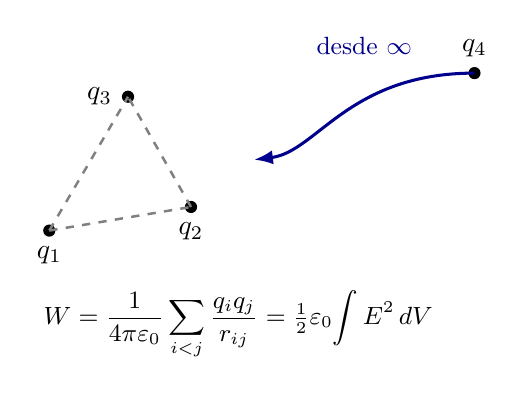
\begin{tikzpicture}[line width=0.9pt,>={Latex[length=2.4mm]}]
  \fill (0,0) circle(2.2pt) node[below=2pt]{$q_1$};
  \fill (1.8,0.3) circle(2.2pt) node[below=2pt]{$q_2$};
  \fill (1.0,1.7) circle(2.2pt) node[left=2pt]{$q_3$};
  \draw[gray,dashed] (0,0)--(1.8,0.3) (0,0)--(1.0,1.7) (1.8,0.3)--(1.0,1.7);
  % q4 viene del infinito
  \fill (5.4,2.0) circle(2.2pt) node[above=2pt]{$q_4$};
  \draw[->,blue!55!black,line width=1.1pt] (5.4,2.0) .. controls (3.8,2.0) and (3.4,1.0) .. (2.6,0.9);
  \node[blue!55!black] at (4.0,2.35){\small desde $\infty$};
  \node at (2.4,-1.2){\small $\displaystyle W=\frac{1}{4\pi\varepsilon_0}\sum_{i<j}\frac{q_i q_j}{r_{ij}}=\tfrac12\varepsilon_0\!\int E^2\,dV$};
\end{tikzpicture}
\end{document}
